\documentclass[11pt]{article}
\title{\textbf{Meccano hexagons}}
\author{https://github.com/heptagons/meccano/hexa}
\date{}

\usepackage{amsmath}
\usepackage{listings}
\usepackage{xcolor}
\definecolor{gray}{RGB}{245,245,245}

\lstset{
	backgroundcolor=\color{gray},
	frame=single,
	language=c,
	numbers=left,
	stepnumber=1
}

\usepackage[margin=0.75in]{geometry}

\usepackage{tikz}
\usetikzlibrary{math}

\usepackage{graphicx}

\begin{document}

\maketitle

\section{Meccano hexagons}

\begin{figure}[htpb]
\centering
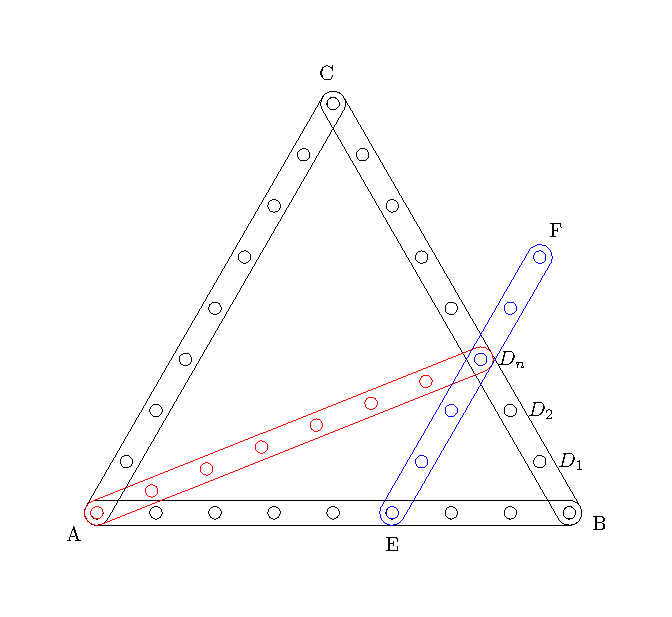
\includegraphics[]{hexagon_angle}
\caption{Regular hexagon internal angle plan. Consider an equilateral triangle $ABC$.
Try to connect a new rod from point $A$ to several points $D$ located 
over the bar $\overline{BC}$
in such a way length $\overline{AD}$ is an integer.
If so, connect a new rod $\overline{EF}$ where $\overline{EB} = \overline{BC}$ and $\overline{EF} = \overline{AE}$. Angle $AEF$ is the internal regular hexagon angle ($120^\circ{}$).}
\label{fig:1}
\end{figure}

Figure \ref{fig:1} shows the regular hexagon internal angle plan.
From the figure the angle at $B$ is fixed to $60^\circ{}$, since $ABC$ is an
rigid equilateral triangle.
Let $a$ and $b$ two integers such as $a >= b/2$.
We are looking for a third integer $d$ called triangle rational diagonal:
\begin{align*}
a &= \overline{AB}\\
b &= \overline{BD}\\
d &= \overline{AD}
\end{align*}

Acording to cosines law, the distance $d$ value is calculated as follows:
\begin{align*}
d^2 &= a^2 + b^2 - 2ab\cos{\frac{\pi}{3}}\\
    &= a^2 + b^2 - ab\\
    &= (a-b)^2 + ab
\end{align*}



\end{document}
